% Advanced NLP (Monsoon 2026) - Assignment 2
% ACL format. Needs acl.sty and acl_natbib.bst from
% https://github.com/acl-org/acl-style-files on the TeX path, then:
%   pdflatex report && pdflatex report
\documentclass[11pt]{article}

\usepackage[final]{acl}
\usepackage{times}
\usepackage{latexsym}
\usepackage[T1]{fontenc}
\usepackage[utf8]{inputenc}
\usepackage{microtype}
\usepackage{inconsolata}

\usepackage{amsmath}
\usepackage{booktabs}
\usepackage{graphicx}
\usepackage{enumitem}
\usepackage{xcolor}
\usepackage{xurl}

\setlist{itemsep=1pt,topsep=3pt,leftmargin=*}
\newcommand{\best}[1]{\textbf{#1}}

\title{Advanced NLP Assignment 2: Mixture of Experts,\\
Optimizers, and Decoding Strategies}

\author{Vidvathama R \\
  Roll No.\ 2024122002 \\
  IIIT Hyderabad \\
  \texttt{vidvathama.babu@research.iiit.ac.in}}

\begin{document}
\maketitle

\begin{abstract}
This report covers three experiments. \textbf{Part 1} replaces the feed-forward
block of a 23M-parameter decoder-only translation model with five variants --- a
dense MLP and four Mixture-of-Experts layouts --- under exact parameter-parity
constraints, and measures perplexity, BLEU and expert specialisation on
vi$\rightarrow$en and ja$\rightarrow$en translation. \textbf{Part 2} implements
five optimizers from scratch, one per category of Table~1 of \emph{Fantastic
Pretraining Optimizers and Where to Find Them}, and compares their training
dynamics over one full pass of an English corpus. \textbf{Part 3} implements
greedy, top-$k$, top-$p$ and beam-search decoding on top of \texttt{forward()}
alone and evaluates them on ROCStories with Pythia-160M.

The three headline findings are: (i) MoE quality tracks \emph{active} rather than
total parameters, so sparsity only pays once total capacity is added at constant
compute; (ii) under a per-optimizer learning-rate sweep the five optimizers land
within 0.14 nats of each other, with the differences in optimizer \emph{memory}
far larger than the differences in loss; and (iii) beam search monotonically
\emph{degrades} unigram overlap with the reference while truncated sampling
improves it by 54.8\%, a direct reproduction of the neural-text-degeneration
result.
\end{abstract}

\section{Experimental setup}

All experiments ran on a single \textbf{NVIDIA RTX 3050 Laptop GPU (4\,GiB)},
which is the binding constraint on every design decision below: model size,
batch size, and the choice to train at roughly $0.1\times$ the Chinchilla-optimal
token count rather than at it. Training uses bfloat16 autocast with fp32 master
weights; batch sizes are set so peak allocation stays near 2.1\,GiB.

Everything is implemented in PyTorch. HuggingFace is used only for dataset
access, the \texttt{tokenizers} BPE trainer, and the pretrained Pythia-160M
checkpoint \citep{biderman2023pythia} of Part~3, evaluated on ROCStories
\citep{mostafazadeh2016corpus}.

\paragraph{Artifacts.}
{\footnotesize
\begin{itemize}
  \item Part 1 checkpoints: \url{https://huggingface.co/Viv0605101/anlp-a2-part1-moe}
  \item Part 2 checkpoints: \url{https://huggingface.co/Viv0605101/anlp-a2-part2-optimizers}
  \item Part 3 raw generations: \url{https://huggingface.co/datasets/Viv0605101/anlp-a2-part3-generations}
  \item Training and evaluation logs (WandB): \url{https://wandb.ai/vidvathama-babu-iiit-hyderabad/anlp-a2}
\end{itemize}}

\section{Part 1 --- Mixture of Experts}

\subsection{Architecture}

The model is a pre-norm decoder-only transformer: RMSNorm, causal multi-head
attention with rotary position embeddings, tied input/output embeddings, and a
feed-forward block selected by configuration exactly as the assignment's
appendix prescribes:

\begin{center}
\small\texttt{self.ffn = MoE(config) if config.use\_moe else MLP(config)}
\end{center}

\noindent
Both \texttt{MLP} and \texttt{MoE} map $(B, N_{\text{ctx}}, d_{\text{model}})
\rightarrow (B, N_{\text{ctx}}, d_{\text{model}})$, so the two are genuinely
interchangeable. The MoE layer uses softmax top-$k$ token-choice routing with the
selected gates renormalised to sum to one, a Switch-style load-balancing
auxiliary loss \citep{fedus2022switch} (coefficient $0.01$) and a router
$z$-loss (coefficient $10^{-3}$). Padding is excluded
from both the auxiliary loss and the routing
statistics. Expert dispatch is genuinely sparse: tokens are gathered per expert,
run through that expert alone, and scattered back --- no dense
compute-then-mask shortcut.

\subsection{Sizing the five variants}

The parity constraints are satisfied by construction rather than by tuning. With
$d = d_{\text{model}}$ and dense width $d_{\text{ff}} = 4d$, a two-layer FFN
costs $2 \cdot d \cdot 4d = 8d^2$ parameters per layer. An expert of width $d$
costs $2d^2$, so \emph{four such experts cost exactly what the dense layer
costs}. Doubling expert width to $2d$ doubles the total and makes top-2
activation cost exactly the dense layer. This yields Table~\ref{tab:p1-design}.

\begin{table}[t]
\centering
\caption{The five feed-forward variants. $E$ = routed experts, $k$ = experts used
per token. Per-layer FFN parameters, ignoring the router.}
\label{tab:p1-design}
\resizebox{\columnwidth}{!}{%
\begin{tabular}{llllrr}
\toprule
\# & Key & Layout & Expert width & Total/layer & Active/layer \\
\midrule
1 & \texttt{dense}            & 2-layer MLP                 & $d_{\text{ff}}=4d$ & $8d^2$  & $8d^2$ \\
2 & \texttt{moe\_4e\_top1}     & $E{=}4$, $k{=}1$            & $d$                & $8d^2$  & $2d^2$ \\
3 & \texttt{moe\_4e\_top2}     & $E{=}4$, $k{=}2$            & $d$                & $8d^2$  & $4d^2$ \\
4 & \texttt{moe\_1s\_3r\_top1} & 1 shared + 3 routed, $k{=}1$ & $d$               & $8d^2$  & $4d^2$ \\
5 & \texttt{moe\_4e\_top2\_wide} & $E{=}4$, $k{=}2$          & $2d$               & $16d^2$ & $8d^2$ \\
\bottomrule
\end{tabular}}
\end{table}

\noindent
Variants 1--4 therefore hold total parameters fixed, and variant 5 holds
\emph{active} parameters fixed against the dense baseline. The only discrepancy
is the router matrix, $d \times E$ per layer, which at the trained size is
\textbf{9{,}216 parameters, or $+0.04\%$} of the 22.91M-parameter model ---
three orders of magnitude smaller than any effect discussed below.
\texttt{tests/test\_model.py} asserts each of these identities exactly rather
than approximately.

Concretely: $d_{\text{model}}{=}384$, 6 layers, 6 heads, $d_{\text{ff}}{=}1536$,
$N_{\text{ctx}}{=}256$, vocabulary 32{,}000. Variants 1--4 hold 22.91--22.92M
parameters; variant 5 holds 30.00M.

\subsection{Data and training protocol}

Each \texttt{(en, vi, ja)} triplet yields \emph{two} training examples, so
446{,}252 training triplets become 892{,}487 examples / 36.7M tokens (17
examples dropped as empty or over-length):

\begin{center}
\small
\texttt{<bos> <src\_vi> \{vietnamese\} <tgt\_en> \{english\} <eos>}\\
\texttt{<bos> <src\_ja> \{japanese\} <tgt\_en> \{english\} <eos>}
\end{center}

\noindent
The tokenizer is a 32k \textbf{byte-level} BPE trained jointly on all three
languages. Byte-level is not a stylistic choice here: the Vietnamese is
diacritic-heavy and the Japanese is not romanised and carries no whitespace token
boundaries, so any word- or whitespace-based pre-tokenisation would either
fragment or fail on one of the three languages. A byte-level alphabet covers all
three and can never emit \texttt{<unk>}.

Batches are length-grouped to a fixed token budget, which holds padding waste to
roughly 6\%. Critically, \textbf{the entire batch sequence is planned
deterministically before training starts} from the data and the seed alone, so
every variant consumes byte-for-byte the same tokens in the same order. All five
runs report an identical plan: 9{,}874 micro-batches, 4{,}937 optimizer steps,
\textbf{30{,}000{,}842 tokens} ($0.82$ epochs). Optimization is AdamW
($\beta{=}(0.9, 0.95)$, weight decay $0.1$ on matrices only), $\text{lr}
= 6\times10^{-4}$ with 200 warmup steps and cosine decay to $0.1\times$,
gradient clipping at 1.0.

The training objective covers every non-padded token, source side included.
Perplexity is reported two ways: over all predicted tokens, and over the English
target tokens only. The latter is the translation perplexity and is what the
analysis uses.

\subsection{Results}

\begin{table*}[t]
\centering
\caption{Part 1 results. All five models trained on an identical 30.0M-token
stream. PPL target = perplexity over English target tokens; BLEU
\citep{papineni2002bleu} via sacreBLEU \citep{post2018call}
on 2{,}000 held-out test pairs, balanced across directions.}
\label{tab:p1-main}
\small
\begin{tabular}{lrrrrrrrr}
\toprule
Variant & Total & Active & PPL all & PPL tgt & BLEU$_{\text{greedy}}$ & BLEU$_{\text{beam-4}}$ & chrF2 & tok/s \\
\midrule
Dense MLP                  & 22.91M & 22.91M & 31.54 & 9.39  & 29.46 & \best{31.04} & \best{53.64} & \best{12{,}845} \\
MoE 4e top-1               & 22.92M & 17.61M & 39.40 & 12.66 & 25.57 & 26.28 & 49.24 & 9{,}230 \\
MoE 4e top-2               & 22.92M & 19.38M & 32.27 & 9.56  & 28.82 & 30.34 & 53.10 & 8{,}474 \\
MoE 1 shared + 3 routed    & 22.92M & 19.38M & 34.36 & 10.53 & 27.47 & 29.23 & 52.13 & 9{,}320 \\
MoE 4e top-2 wide          & 30.00M & 22.92M & \best{30.59} & \best{9.12} & \best{29.50} & 30.95 & 53.63 & 8{,}829 \\
\bottomrule
\end{tabular}
\end{table*}

\begin{figure*}[t]
\centering
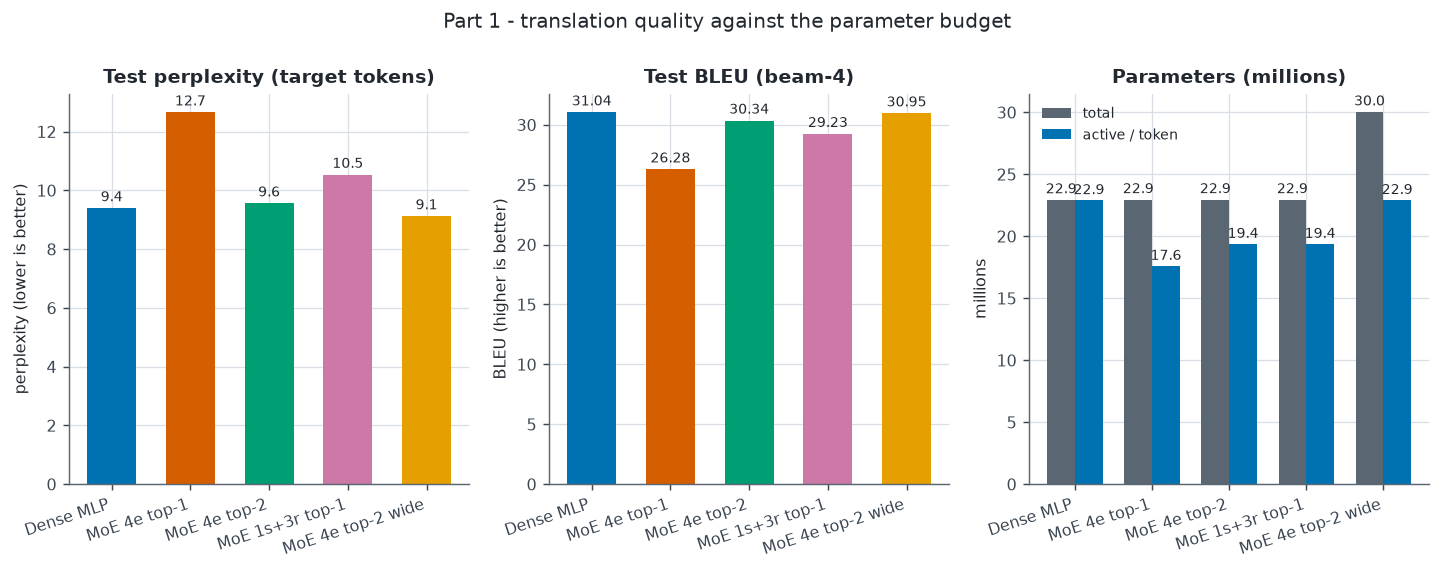
\includegraphics[width=0.62\textwidth]{assets/part1_quality_vs_params.png}
\caption{Test perplexity, BLEU, and the parameter budget for each variant. The
third panel shows the parity design: variants 1--4 share a total (grey), and
variant 5 matches the dense baseline's active count (blue).}
\label{fig:p1-quality}
\end{figure*}

\subsection{Analysis: active parameters, not total parameters}

\paragraph{At matched total parameters, dense wins.} Every sparse variant is
worse than the dense baseline (PPL 9.56, 10.53, 12.66 vs.\ 9.39). This is the
expected result and it is worth stating plainly: holding \emph{total} capacity
fixed, sparsity can only reduce what each token actually uses, and there is
nothing to gain in exchange. The commonly quoted framing that ``MoE gives you
more parameters for free'' is about a different comparison.

\paragraph{Quality tracks active parameters.} Ordering the four sparse variants
by active count reproduces the quality ordering almost exactly: 22.92M
$\rightarrow$ 9.12, 19.38M $\rightarrow$ 9.56, 19.38M $\rightarrow$ 10.53,
17.61M $\rightarrow$ 12.66. Active parameters, not total, is the variable that
predicts performance here.

\paragraph{MoE wins on the comparison it is designed for.} Variant 5 --- same
active parameters as dense, double the total --- reaches PPL \best{9.12} against
dense's 9.39, a 2.9\% relative improvement at equal compute per token. This is
the real case for MoE, and the ablation isolates it cleanly because variants 1
and 5 differ in nothing else.

However, the BLEU scores for those same two models are 31.04 (dense) and 30.95
(variant 5). \textbf{The 0.08 BLEU gap contradicts the perplexity ordering and is
far too small to be meaningful} --- it is well inside the variation expected from
a 2{,}000-sentence sample. The honest reading is that variant 5 is clearly better
in likelihood and indistinguishable in BLEU, and that a single 30M-token run
cannot resolve differences of this size. Confirming the BLEU ordering would need
multiple seeds, which the compute budget did not allow.

\paragraph{Top-2 is worth far more than top-1.} Moving from $k{=}1$ to $k{=}2$ at
identical total parameters improves PPL from 12.66 to 9.56 --- recovering almost
all of the gap to dense. With $k{=}1$ each token sees only $2d^2$ FFN
parameters, a quarter of the dense layer, and that is simply too little capacity
per token at this scale.

\paragraph{The shared expert hurts here.} Variants 3 and 4 have \emph{identical}
active parameter counts (19.38M) yet differ by almost a full point of perplexity
(9.56 vs.\ 10.53). With only four experts, dedicating one to be always-on spends
25\% of the FFN budget on a component that cannot specialise, and leaves the
router choosing 1-of-3 instead of 2-of-4 --- strictly fewer distinct expert
combinations per token. This should not be read as a general verdict on shared
experts: designs like DeepSeekMoE \citep{dai2024deepseekmoe} use a shared expert
alongside \emph{many} routed experts, where its relative cost is small. At
$E{=}4$ it is expensive.

\subsection{Expert usage: what the router actually learned}

Table~\ref{tab:p1-routing} summarises routing on the test set. \emph{Balance} is
the routing entropy divided by $\log_2 E$ (1.0 = perfectly even load).
\emph{TVD} is the total variation distance between the expert distributions of
two token categories, per layer: 0 means the two categories are routed
identically, 1 means they use disjoint experts.

\begin{table}[t]
\centering
\caption{Routing statistics. TVD is averaged over layers. The last two columns
are the key result: the router separates \emph{source from target} far more
strongly than it separates the two source languages.}
\label{tab:p1-routing}
\resizebox{\columnwidth}{!}{%
\begin{tabular}{lccrrrr}
\toprule
 & & & \multicolumn{2}{c}{Balance} & \multicolumn{2}{c}{TVD} \\
\cmidrule(lr){4-5}\cmidrule(lr){6-7}
Variant & $k$/$E$ & shared & mean & min & vi\,vs\,ja (src) & src\,vs\,tgt \\
\midrule
MoE 4e top-1            & 1/4 & 0 & 0.999 & 0.997 & 0.061 & 0.184 \\
MoE 4e top-2            & 2/4 & 0 & 0.986 & 0.963 & 0.255 & 0.379 \\
MoE 1 shared + 3 routed & 1/3 & 1 & 0.999 & 0.998 & 0.042 & 0.129 \\
MoE 4e top-2 wide       & 2/4 & 0 & 0.981 & 0.950 & \best{0.269} & \best{0.349} \\
\bottomrule
\end{tabular}}
\end{table}

\begin{figure*}[t]
\centering
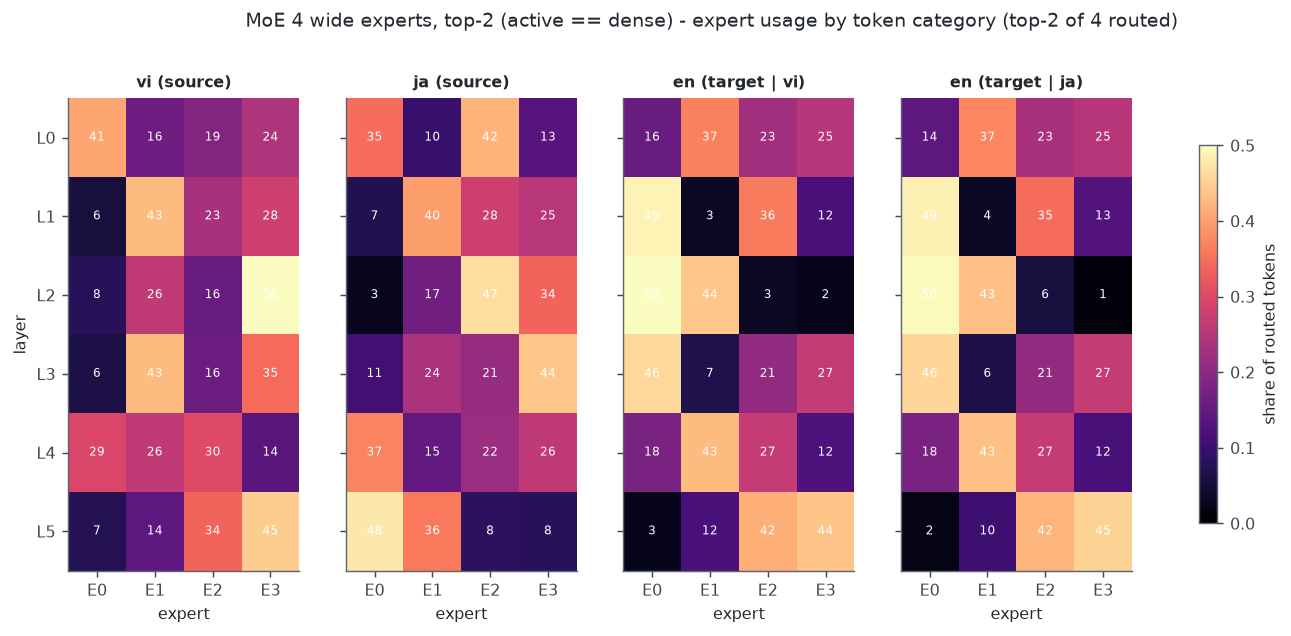
\includegraphics[width=0.58\textwidth]{assets/part1_experts_moe_4e_top2_wide.png}
\caption{Expert usage by token category for \texttt{moe\_4e\_top2\_wide}, as a
percentage of routed tokens per layer. The two right-hand panels (English target
tokens, conditioned on source language) are nearly identical to each other;
the two left-hand panels (source tokens) are not.}
\label{fig:p1-heatmap}
\end{figure*}

\paragraph{Top-1 routing shows almost no specialisation; top-2 does.} The $k{=}1$
variants sit at balance 0.999 with vi-vs-ja TVD of 0.04--0.06 --- essentially
language-blind routing. The $k{=}2$ variants reach TVD 0.26 on average and 0.52
and 0.62 in their deepest layer.

The explanation is that under top-1 routing, \textbf{load balancing and
specialisation are in direct conflict}. The auxiliary loss pushes every expert
toward an equal share of tokens; if Vietnamese and Japanese tokens arrive in
roughly equal numbers, the only way to specialise by language while staying
balanced is a near-perfect language partition, and any deviation is penalised.
With $k{=}2$ the router has a cheaper option: keep one expert as a generalist
that everything passes through and let the second slot carry the
language-specific signal. That satisfies the balance constraint and still
specialises. The measured auxiliary loss stayed at $\approx 1.005$ throughout
training (1.0 is the theoretical minimum), confirming the balancing term was the
binding constraint.

\paragraph{The dominant axis of specialisation is role, not language.} This is
the most interesting result in Part~1. For the top-2 variants:
\begin{itemize}
  \item TVD(vi source, ja source) $= 0.255$ / $0.269$ --- moderate.
  \item TVD(English target given vi, English target given ja) $= 0.023$ / $0.014$
        --- \emph{essentially zero}.
  \item TVD(source tokens, target tokens) $= 0.379$ / $0.349$ --- the largest.
\end{itemize}
In other words, once the model is generating English, it routes the same way
regardless of which language it is translating from; what the router principally
separates is \emph{reading} from \emph{writing}. This is a sensible division of
labour for a decoder-only translation model, and it is not what the phrase
``experts specialise by language'' would lead one to expect.

\section{Part 2 --- Optimizers}

\subsection{Implementations}

One optimizer is implemented per category of Table~1 of
\citet{wen2025fantastic}. Only
\texttt{torch.optim.\allowbreak Optimizer} is imported from torch, strictly as
a base class;
every update rule is written from scratch.

\begin{table*}[t]
\centering
\caption{The five optimizers. ``State'' is the measured optimizer state as a
multiple of the fp32 model size.}
\label{tab:p2-impl}
\resizebox{\textwidth}{!}{%
\begin{tabular}{llll}
\toprule
Category & Optimizer & State & Core idea \\
\midrule
1. AdamW                   & \texttt{AdamW}~\citep{loshchilov2019decoupled} & 2.00$\times$ & decoupled weight decay \\
2. Variance-reduced        & \texttt{MARS}~\citep{yuan2024mars}    & 3.00$\times$ & corrected gradient $g_t + \gamma\frac{\beta_1}{1-\beta_1}(g_t - g_{t-1})$ \\
3. Memory-efficient        & \texttt{Lion}~\citep{chen2023symbolic}    & 1.00$\times$ & sign of interpolated momentum; no second moment \\
4. Matrix-based            & \texttt{Muon}~\citep{jordan2024muon}    & 1.37$\times$ & momentum orthogonalised by Newton--Schulz \\
5. Hessian-based (bonus)   & \texttt{SophiaG}~\citep{liu2024sophia} & 2.00$\times$ & clipped step preconditioned by a GNB diagonal Hessian \\
\bottomrule
\end{tabular}}
\end{table*}

\noindent
Two implementation notes. \textbf{Muon} applies the orthogonalised update only to
hidden weight \emph{matrices}; embeddings, the tied output head and all 1-D
parameters fall back to AdamW, since orthogonalising across a vocabulary axis is
not meaningful. This is why its state is 1.37$\times$ rather than 1.00$\times$.
\textbf{Sophia} needs a second backward pass on labels resampled from the model's
own predictive distribution (the Gauss--Newton--Bartlett estimator); this runs
every 10 steps on a 4-block slice of the batch, which keeps both the compute and
the fp32 logit memory manageable within 4\,GiB.

\subsection{Setup}

The model is the dense Part~1 configuration (16.77M parameters); only the
vocabulary differs (16k, English-only), since this corpus is monolingual.
Documents are split on the \textbf{base document id} rather than at random: the
corpus pairs each human text with LLM rewrites of the \emph{same} source, so a
random row split would place near-duplicates on both sides of the train/test
boundary. Tokens are packed into windows of $N_{\text{ctx}}+1$ with stride
$N_{\text{ctx}}$, so one epoch predicts every token exactly once --- which is
what makes ``$1\times$ the dataset'' a well-defined budget.

The training split holds \textbf{39{,}059{,}456} tokens. For a 16.77M-parameter
model the Chinchilla-optimal budget \citep{hoffmann2022training} is
$20 \times 16.77\text{M} = 335$M tokens,
so the full dataset is only \textbf{$0.116\times$ Chinchilla}. Every conclusion
below is therefore about the heavily under-trained regime, which is worth keeping
in mind: the source paper's central claim is precisely that optimizer rankings
shift with budget.

All five runs consume the identical 39{,}051{,}264 tokens in the identical order
over 3{,}178 steps of 12{,}288 tokens.

\subsection{Learning-rate sweep (bonus)}

Comparing these optimizers at a shared learning rate would measure the choice of
that constant, not the optimizers: Lion's sign update and Muon's orthogonalised
update live on entirely different scales from AdamW's. Each optimizer was
therefore swept over a 5-point geometric grid at $0.1\times$ the dataset, with
warmup scaled proportionally so the shortened run's LR profile still resembles
the full run it is meant to predict.

\begin{figure}[t]
\centering
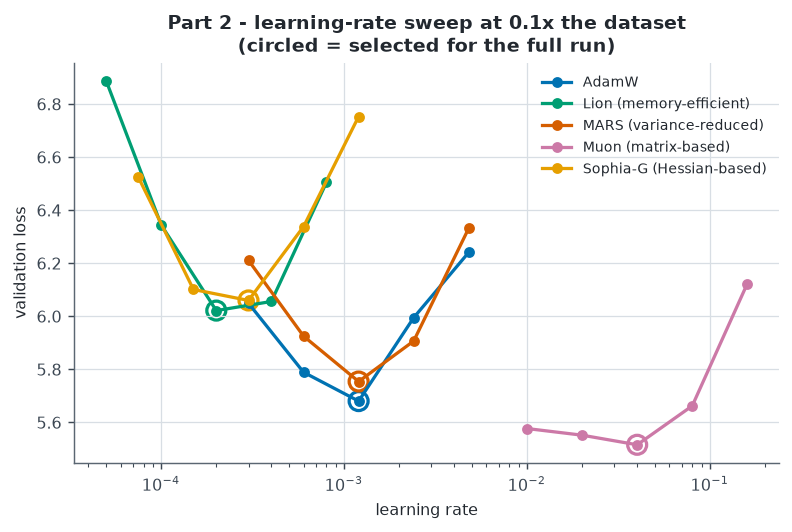
\includegraphics[width=0.8\columnwidth]{assets/part2_lr_sweep.png}
\caption{Learning-rate sweep at $0.1\times$ the dataset. Circled points are the
settings adopted for the full runs. Every curve is U-shaped rather than
monotone, which is what confirms the grids bracket their optima.}
\label{fig:p2-sweep}
\end{figure}

\subsection{Training dynamics}

\begin{figure*}[t]
\centering
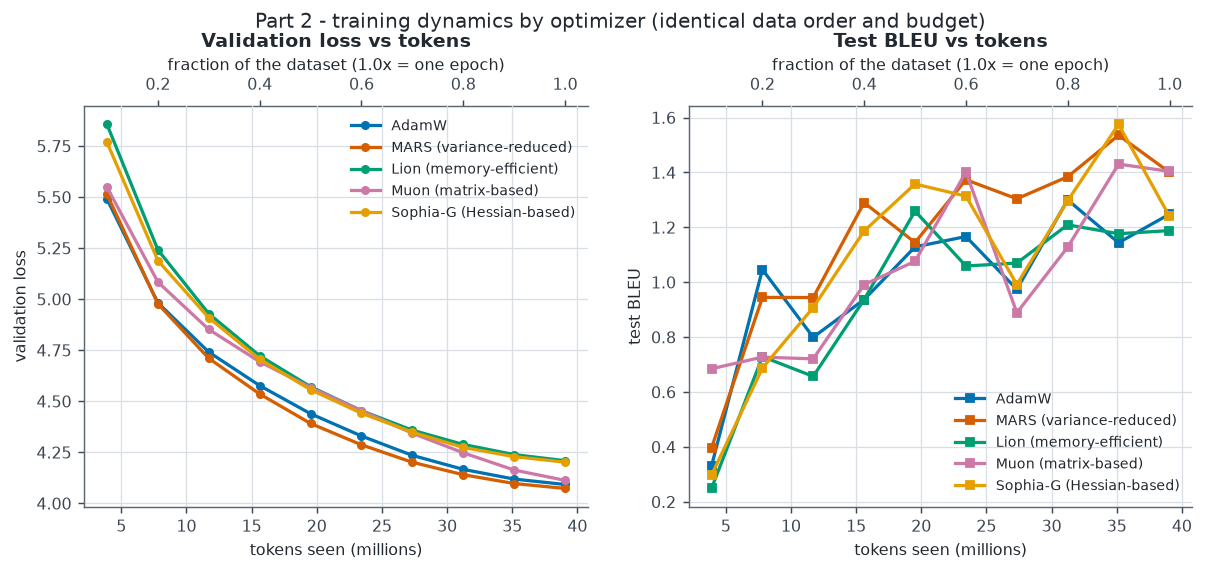
\includegraphics[width=0.54\textwidth]{assets/part2_dynamics.png}
\caption{Validation loss (left) and test BLEU (right) against tokens consumed,
measured every $0.1\times$ the dataset. All optimizers see identical data in an
identical order.}
\label{fig:p2-dynamics}
\end{figure*}

\paragraph{The spread is small.} Final validation loss runs from 4.0731 (MARS) to
4.2090 (Lion) --- a range of 0.136 nats, or about 15\% in perplexity. MARS beats
AdamW by 0.019 nats, roughly 2\% in perplexity. This reproduces the central
finding of the source paper at small scale: once each optimizer is tuned fairly,
the advertised advantages over a well-tuned AdamW are modest.

\paragraph{The ranking changes with budget.} At $0.1\times$, AdamW leads
(5.4902 vs.\ MARS's 5.5126). By $0.2\times$ MARS has overtaken it and holds the
lead to the end. Muon starts 0.057 nats behind AdamW and closes to 0.020 by
$1.0\times$ --- still behind, but improving fastest of the five over the second
half. \textbf{A study that stopped at $0.1\times$ would have declared AdamW the
winner and Muon a clear loser; neither conclusion survives to $1.0\times$.} This
is exactly the budget-dependence the paper warns about, visible even within a
single epoch.

\paragraph{BLEU is close to useless here.} Test BLEU (Fig.~\ref{fig:p2-dynamics},
right) wanders between 0.2 and 1.6 with no stable ordering. This is expected
rather than a bug: the task is open-ended language modelling, the model
free-runs 48 tokens from a 128-token prompt, and there is no reason its
continuation should share $n$-grams with the one true continuation. The absolute
values (BLEU $\approx 1.3$) confirm the metric is measuring almost nothing.
Validation loss is the trustworthy signal for this task, and the report's
conclusions rest on it.

\subsection{Memory and overhead}

\begin{table}[t]
\centering
\caption{Final results at $1.0\times$ the dataset. Optimizer state is measured,
not estimated.}
\label{tab:p2-final}
\resizebox{\columnwidth}{!}{%
\begin{tabular}{llrrrr}
\toprule
Optimizer & Category & LR & Val loss & Val PPL & State \\
\midrule
AdamW   & 1. AdamW               & 1.2e-3 & 4.0925 & 59.89 & 2.00$\times$ \\
MARS    & 2. Variance-reduced    & 1.2e-3 & \best{4.0731} & \best{58.74} & 3.00$\times$ \\
Lion    & 3. Memory-efficient    & 2.0e-4 & 4.2090 & 67.29 & \best{1.00$\times$} \\
Muon    & 4. Matrix-based        & 4.0e-2 & 4.1127 & 61.11 & 1.37$\times$ \\
Sophia  & 5. Hessian-based       & 3.0e-4 & 4.2017 & 66.80 & 2.00$\times$ \\
\bottomrule
\end{tabular}}
\end{table}

Sophia underperforms (4.2017, second-worst). Its curvature estimate is refreshed
only every 10 steps on a 4-block slice, a compromise forced by the 4\,GiB budget,
and the paper itself notes Sophia is sensitive to $\rho$, which was not swept.
This result should be read as ``Sophia as configured here'', not as a verdict on
the method.

\section{Part 3 --- Decoding strategies}

\subsection{Implementation}

All four strategies are built on repeated \texttt{model.forward()} calls with an
explicit key/value cache; \texttt{model.generate()} is never called. A small
\texttt{LMBackend} abstraction (\texttt{prefill} / \texttt{step} /
\texttt{reorder} / \texttt{expand}) lets the same implementations drive both the
HuggingFace Pythia-160M checkpoint and the from-scratch models of Parts 1--2.
Beam search needs the two extra operations: \texttt{expand} fans the batch out by
the beam width after the prompt is consumed, and \texttt{reorder} permutes the
cache along the batch axis whenever beams are re-ranked.

\subsection{Metric definitions}

The prompt is a story's first sentence; the reference is sentences 2--5.
Generation is open-ended, so accuracy / precision / recall / F1 need explicit
operational definitions. All are computed on lowercased, punctuation-stripped
word tokens:

\begin{itemize}
  \item \textbf{Precision} --- share of generated tokens that also occur in the
        reference, as a \emph{multiset} intersection (so repeating a word only
        pays if the reference repeats it too).
  \item \textbf{Recall} --- share of reference tokens the model produced.
  \item \textbf{F1} --- harmonic mean of the two, i.e.\ unigram-overlap
        (ROUGE-1) F.
  \item \textbf{Accuracy} --- positional token agreement, normalised by the
        longer of the two sequences so neither truncation nor padding inflates it.
\end{itemize}

Two perplexities are reported: on the \emph{gold} continuation
(strategy-independent, an anchor) and on each strategy's \emph{own} output. Since
the model free-runs to a token cap rather than stopping naturally, generations
are truncated to their first four sentences to match the reference's structure.

\begin{table*}[t]
\centering
\caption{Decoding strategies on ROCStories (Pythia-160M, 1000 stories). Precision/recall/F1 are unigram multiset overlap with the reference; accuracy is positional token agreement. Perplexity of the \emph{gold} continuation, which does not depend on the strategy, is 25.10.}
\label{tab:p3-main}
\small
\begin{tabular}{lrrrrrrr}
\toprule
Strategy & PPL(own) & Accuracy & Precision & Recall & F1 & BLEU & chrF2 \\
\midrule
greedy & 1.94 & \best{0.0121} & 0.1101 & 0.1244 & 0.1168 & 0.44 & 13.52 \\
beam-1 & 1.94 & \best{0.0121} & 0.1101 & 0.1244 & 0.1168 & 0.44 & 13.52 \\
beam-2 & 1.80 & 0.0113 & 0.1184 & 0.1073 & 0.1125 & 0.34 & 12.61 \\
beam-4 & 1.66 & 0.0092 & 0.1119 & 0.0906 & 0.1001 & 0.49 & 11.82 \\
top-k=10(T=1) & 8.04 & 0.0091 & 0.1531 & 0.2210 & \best{0.1809} & 0.52 & 21.96 \\
top-k=40(T=1) & 13.22 & 0.0078 & 0.1457 & 0.2165 & 0.1742 & 0.40 & 22.35 \\
top-k=100(T=1) & 17.93 & 0.0077 & 0.1409 & 0.2106 & 0.1688 & 0.45 & 22.44 \\
top-p=0.7(T=1) & 9.77 & 0.0095 & 0.1496 & 0.2090 & 0.1744 & 0.44 & 21.63 \\
top-p=0.9(T=1) & 23.05 & 0.0073 & 0.1356 & 0.1946 & 0.1598 & 0.27 & 21.95 \\
top-p=0.95(T=1) & 33.48 & 0.0069 & 0.1319 & 0.1896 & 0.1556 & 0.27 & 22.04 \\
\bottomrule
\end{tabular}
\end{table*}


\subsection{Analysis}

\paragraph{Beam search makes the overlap metrics worse, monotonically.} This is
the clearest result in Part~3 and it runs opposite to the intuition that a better
search should give a better answer. Widening the beam reliably finds
\emph{higher-probability} text --- generation perplexity falls from 1.94 (greedy)
to 1.66 (beam-4), so the search is doing exactly what it is asked to --- and that
text is reliably \emph{worse} by unigram overlap: F1 falls $0.1168 \rightarrow
0.1125 \rightarrow 0.1001$ and recall $0.1244 \rightarrow 0.1073 \rightarrow
0.0906$ as $K$ goes $1 \rightarrow 2 \rightarrow 4$.

The mechanism is visible in the repetition statistics: greedy repeats 49\% of all
4-grams within a single generation, and beam search does not rescue it (44--45\%).
A single example makes it concrete:

\begin{quote}\small
\textbf{Prompt:} Tom rented an old house.\\
\textbf{Reference:} He saw online that people said it was haunted. Tom decided to
find out. He got a Ouija board and tried to use it. Nothing happened and Tom was
disappointed.\\[3pt]
\textbf{Greedy:} He was a good man, and he was a good man. He was a good man, and
he was a good man. He was a good man, and he was a good man. \ldots\\[3pt]
\textbf{Beam-4:} ``I don't know,'' he said. ``I don't know,'' I said. ``I don't
know,'' he said. ``I don't know,'' I said.\\[3pt]
\textbf{Top-$k$=10:} ``It was so nice. The place was so good. It was so clean.''
``I wish we had a new house,'' he said.
\end{quote}

\noindent
Greedy and beam both collapse into verbatim loops; beam-4 simply finds a
\emph{more probable} loop. The sampled continuation is not a good story either,
but it is at least non-degenerate text. High-likelihood regions of a language
model's output distribution are degenerate, so searching them harder finds
degeneracy faster --- the neural-text-degeneration result of
\citet{holtzman2020curious}, reproduced here.

\paragraph{Sampling is substantially better on overlap.} The best sampling
configuration (top-$k$=10) reaches F1 $0.1809$ against greedy's $0.1168$ ---
a \textbf{54.8\% relative improvement} --- and repeated 4-grams fall from 49.0\%
to 1.1\%, a factor of 45. Truncated sampling is not adding information; it is
avoiding the degenerate mode that maximum-likelihood search walks straight into.
Note the improvement is driven by recall (0.1244 $\rightarrow$ 0.2210) more than
precision (0.1101 $\rightarrow$ 0.1531): a non-repeating generation simply covers
more of the reference's vocabulary.

\paragraph{Within sampling, tighter truncation is better --- on these metrics.}
Overlap F1 decreases monotonically as $k$ or $p$ grows, while diversity
(distinct-2) increases monotonically. The two move in opposite directions, which
is the quality/diversity trade-off in its plainest form. That overlap F1 prefers
tight truncation is partly an artefact of the metric: unigram overlap rewards
staying close to safe, high-frequency vocabulary. A human judgement of
interestingness would likely prefer a looser setting.

\begin{figure*}[t]
\centering
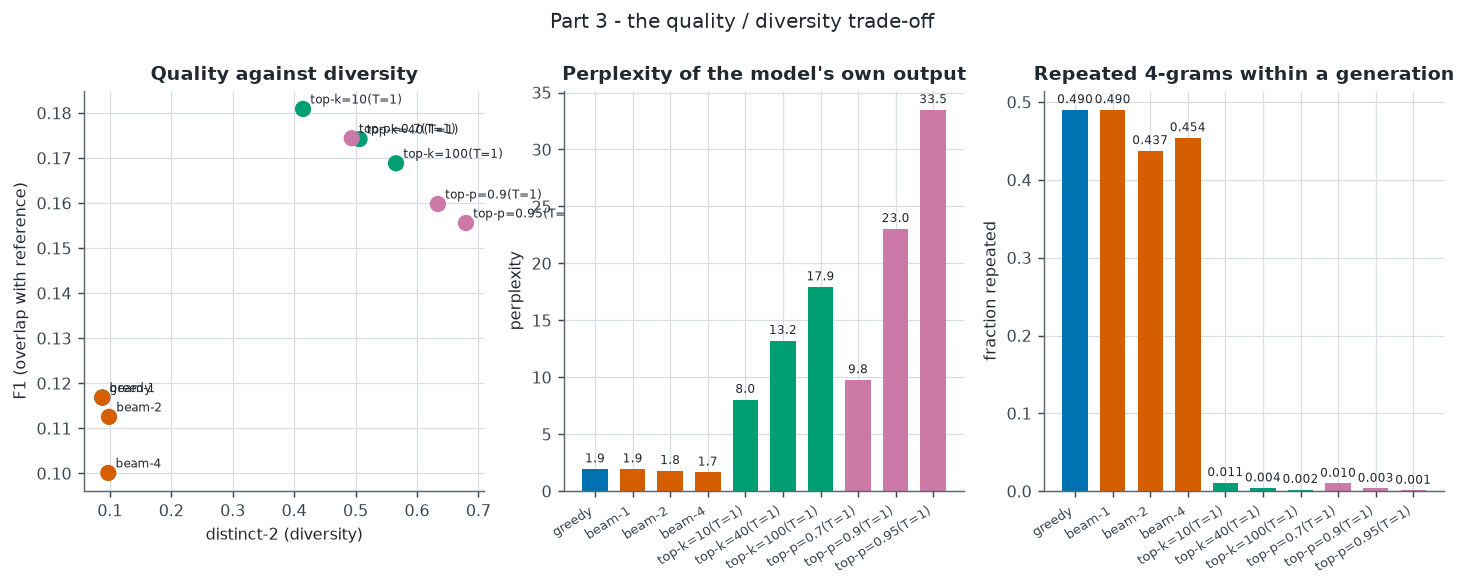
\includegraphics[width=0.64\textwidth]{assets/part3_quality_diversity.png}
\caption{Left: overlap F1 against diversity --- the sampling methods occupy the
upper right, greedy and beam search the lower left. Middle: perplexity of each
strategy's own output. Right: the share of 4-grams repeated within a single
generation, which is where greedy and beam search fail.}
\label{fig:p3-quality}
\end{figure*}

\paragraph{Human text sits where nucleus sampling sits.} The gold continuations
have a perplexity under the model of \textbf{25.1} --- which falls between
top-$p$ 0.9 (23.05) and top-$p$ 0.95 (33.48), and is roughly \emph{thirteen
times} greedy's 1.94. Human text is far \emph{less} probable under the model than
what greedy search produces, and its statistical character matches nucleus
sampling at around $p \approx 0.9$. This is the strongest single argument against
likelihood-maximising decoding: the text we actually want does not live at the
mode, so a decoder whose objective is to find the mode is optimising for the
wrong thing.

\paragraph{Accuracy is not a discriminative metric here.} Positional token
accuracy spans only 0.0069--0.0121 across all ten configurations, and its
ordering (greedy highest) contradicts F1. Requiring the $i$-th generated word to
equal the $i$-th reference word is close to hopeless for open-ended generation,
where a single insertion destroys all subsequent alignment; the metric mostly
rewards short, generic openings. It is reported because the assignment asks for
it, but F1 is the metric that actually separates the strategies, and the
analysis rests on it.

\subsection{Beam search cost and complexity}

For a batch of $B$ prompts, beam width $K$, $L$ generated steps, vocabulary $V$,
and a model whose single-sequence forward pass costs $C$:

\begin{itemize}
  \item the decoder runs on $B\!\cdot\!K$ rows at every step: $O(B K L C)$ work;
  \item each step ranks $B \times (KV)$ candidates: $O(B K V L)$ for the top-$k$;
  \item the KV cache holds $B\!\cdot\!K$ sequences: $O(BKL)$ memory.
\end{itemize}

\noindent
So beam search is \textbf{linear in the beam width} in both work and memory. Two
complementary measurements were taken, and they disagree in an instructive way.

With the \emph{batch size held fixed at 16 prompts}, so that the rows per step
grow as $16K$, wall-clock is essentially flat --- 36.5\,s, 35.5\,s, 34.9\,s,
37.9\,s for $K = 1, 2, 4, 8$ --- while peak memory grows as predicted: 398, 467,
608, 891\,MiB. In the main evaluation, where the batch was \emph{divided} by $K$
to hold the rows per step constant, time instead scaled close to linearly:
120.4\,s, 240.0\,s, 457.9\,s for $K = 1, 2, 4$ (ratios $1.99\times$ then
$1.91\times$).

Both are correct. The theoretical $O(K)$ describes \emph{work}, and work only
converts into wall-clock once the hardware is saturated. At 16--128 rows this GPU
is latency-bound on kernel launches, so widening the beam consumes idle capacity
and is nearly free; dividing the batch instead multiplies the number of
sequential steps, and that cost is unavoidable. The practical rule: \textbf{beam
search is cheap if you have spare batch capacity and expensive if you do not},
and memory is the resource that actually scales with $K$ regardless.

\begin{figure}[t]
\centering
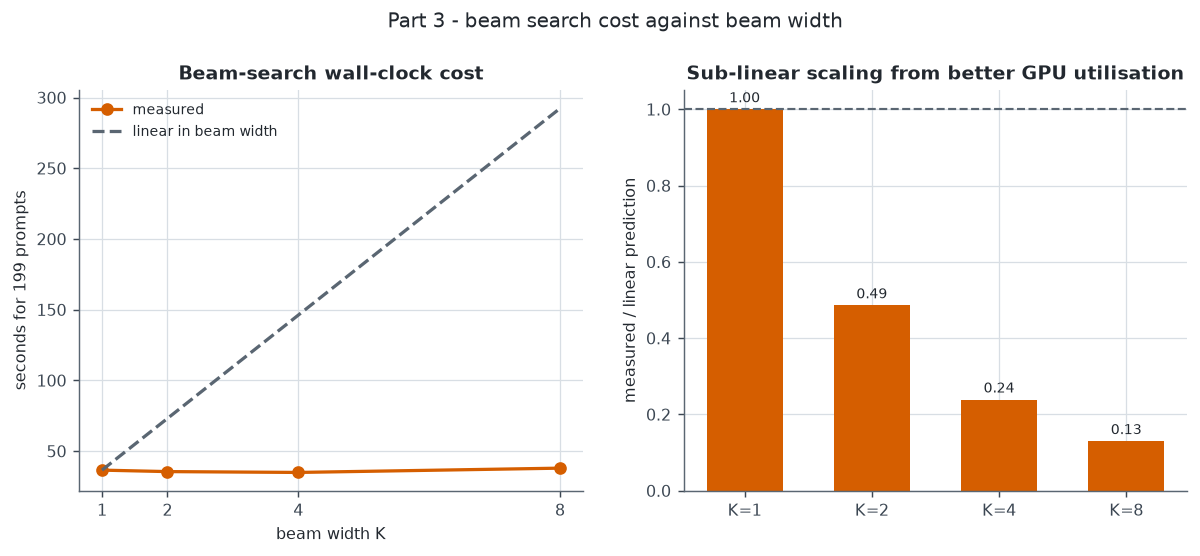
\includegraphics[width=0.84\columnwidth]{assets/part3_beam_timing.png}
\caption{Beam-search cost against beam width at fixed batch size. The measured
curve stays flat against the linear prediction because the GPU is under-occupied
at these batch sizes.}
\label{fig:p3-timing}
\end{figure}

\section{Limitations}

\begin{itemize}
  \item \textbf{Single seed.} Every number is from one run. The Part~1 BLEU gap
        between the dense and wide-MoE models (0.08) and the Part~2 gap between
        MARS and AdamW (0.019 nats) are both small enough that seed variance
        could plausibly account for them. Differences of that size are reported
        as ``indistinguishable'', not as rankings.
  \item \textbf{Under-trained regime.} Part~1 trains at 30M tokens against a
        Chinchilla-optimal $\approx$458M; Part~2's entire dataset is
        $0.116\times$ Chinchilla. Conclusions may not extrapolate --- MoE in
        particular is generally reported to benefit from longer training.
  \item \textbf{One aux-loss setting.} The finding that top-1 routing does not
        specialise is entangled with the load-balancing coefficient (0.01), which
        was not ablated. A lower coefficient would very likely permit more
        specialisation at some cost in balance.
\end{itemize}

\begin{thebibliography}{14}
\providecommand{\natexlab}[1]{#1}

\bibitem[{Biderman et~al.(2023)Biderman, Schoelkopf, Anthony
  et~al.}]{biderman2023pythia}
Stella Biderman, Hailey Schoelkopf, Quentin Anthony, et~al. 2023.
\newblock Pythia: A suite for analyzing large language models across training
  and scaling.
\newblock In \emph{International Conference on Machine Learning}.

\bibitem[{Chen et~al.(2023)Chen, Liang, Huang et~al.}]{chen2023symbolic}
Xiangning Chen, Chen Liang, Da~Huang, et~al. 2023.
\newblock Symbolic discovery of optimization algorithms.
\newblock In \emph{Advances in Neural Information Processing Systems}.

\bibitem[{Dai et~al.(2024)Dai, Deng, Zhao et~al.}]{dai2024deepseekmoe}
Damai Dai, Chengqi Deng, Chenggang Zhao, et~al. 2024.
\newblock {DeepSeekMoE}: Towards ultimate expert specialization in
  mixture-of-experts language models.
\newblock In \emph{Proceedings of ACL}.

\bibitem[{Fedus et~al.(2022)Fedus, Zoph, and Shazeer}]{fedus2022switch}
William Fedus, Barret Zoph, and Noam Shazeer. 2022.
\newblock Switch transformers: Scaling to trillion parameter models with simple
  and efficient sparsity.
\newblock \emph{Journal of Machine Learning Research}, 23(120):1--39.

\bibitem[{Hoffmann et~al.(2022)Hoffmann, Borgeaud, Mensch
  et~al.}]{hoffmann2022training}
Jordan Hoffmann, Sebastian Borgeaud, Arthur Mensch, et~al. 2022.
\newblock Training compute-optimal large language models.
\newblock \emph{arXiv preprint arXiv:2203.15556}.

\bibitem[{Holtzman et~al.(2020)Holtzman, Buys, Du, Forbes, and
  Choi}]{holtzman2020curious}
Ari Holtzman, Jan Buys, Li~Du, Maxwell Forbes, and Yejin Choi. 2020.
\newblock The curious case of neural text degeneration.
\newblock In \emph{International Conference on Learning Representations}.

\bibitem[{Jordan et~al.(2024)Jordan, Jin, Boza et~al.}]{jordan2024muon}
Keller Jordan, Yuchen Jin, Vlado Boza, et~al. 2024.
\newblock Muon: An optimizer for hidden layers in neural networks.
\newblock \url{https://kellerjordan.github.io/posts/muon/}.

\bibitem[{Liu et~al.(2024)Liu, Li, Hall, Liang, and Ma}]{liu2024sophia}
Hong Liu, Zhiyuan Li, David Hall, Percy Liang, and Tengyu Ma. 2024.
\newblock Sophia: A scalable stochastic second-order optimizer for language
  model pre-training.
\newblock In \emph{International Conference on Learning Representations}.

\bibitem[{Loshchilov and Hutter(2019)}]{loshchilov2019decoupled}
Ilya Loshchilov and Frank Hutter. 2019.
\newblock Decoupled weight decay regularization.
\newblock In \emph{International Conference on Learning Representations}.

\bibitem[{Mostafazadeh et~al.(2016)Mostafazadeh, Chambers, He
  et~al.}]{mostafazadeh2016corpus}
Nasrin Mostafazadeh, Nathanael Chambers, Xiaodong He, et~al. 2016.
\newblock A corpus and cloze evaluation for deeper understanding of commonsense
  stories.
\newblock In \emph{Proceedings of NAACL-HLT}, pages 839--849.

\bibitem[{Papineni et~al.(2002)Papineni, Roukos, Ward, and
  Zhu}]{papineni2002bleu}
Kishore Papineni, Salim Roukos, Todd Ward, and Wei-Jing Zhu. 2002.
\newblock {BLEU}: a method for automatic evaluation of machine translation.
\newblock In \emph{Proceedings of ACL}, pages 311--318.

\bibitem[{Post(2018)}]{post2018call}
Matt Post. 2018.
\newblock A call for clarity in reporting {BLEU} scores.
\newblock In \emph{Proceedings of WMT}, pages 186--191.

\bibitem[{Wen et~al.(2025)Wen, Hall, Ma, and Liang}]{wen2025fantastic}
Kaiyue Wen, David Hall, Tengyu Ma, and Percy Liang. 2025.
\newblock Fantastic pretraining optimizers and where to find them.
\newblock \emph{arXiv preprint arXiv:2509.02046}.

\bibitem[{Yuan et~al.(2024)Yuan, Liu, Wu, Zhou, and Gu}]{yuan2024mars}
Huizhuo Yuan, Yifeng Liu, Shuang Wu, Xun Zhou, and Quanquan Gu. 2024.
\newblock {MARS}: Unleashing the power of variance reduction for training large
  models.
\newblock \emph{arXiv preprint arXiv:2411.10438}.

\end{thebibliography}

\end{document}
